\chapter{Lecture 12: Contour Integrals}

\begin{example}
    Compute:
    $$\int_{0}^{\infty} \frac{\sin^2 x}{x^2} dx$$

    \textbf{step 1:} Replace with a complex function:
    \begin{align*}
        2\sin^2 x                                 & = 1 - \cos 2x                                                                       \\
        \int_{0}^{\infty} \frac{\sin^2 x}{x^2} dx & = \frac{1}{2} \int_{-\infty}^{\infty} \frac{\sin^2 x}{x^2} dx                       \\
                                                  & = \frac{1}{4} \int_{-\infty}^{\infty} \frac{1 - \cos 2x}{x^2} dx                    \\
                                                  & = \frac{1}{4} \int_{-\infty}^{\infty} \frac{1 - \cos 2z}{z^2} dz                    \\
                                                  & = \Re \left( \frac{1}{4} \int_{-\infty}^{\infty} \frac{1 - e^{2iz}}{z^2} dz \right)
    \end{align*}

    \textbf{step 2:} Choose the right contour:
    Previously, we used a semi-circle in the upper half plane with the condition that there are no zeroes on the line $Im(z) = 0$. This time, there is a zero at $z = 0$. So, we need to use a contour that excludes this zero. We can use a semi-circle in the upper half plane with a small semi-circle around the origin removed (half-keyhole contour) as seen in the figure below.
    \begin{figure}[H]
        \centering
        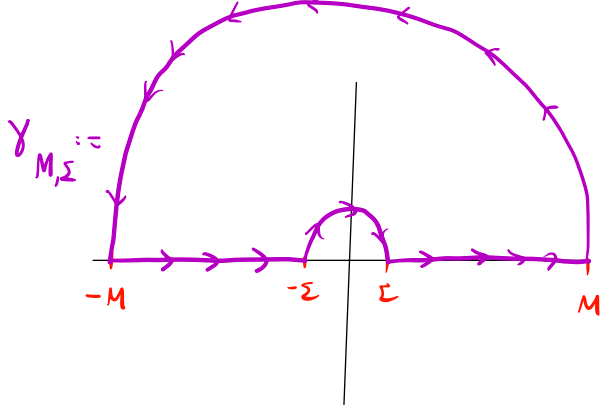
\includegraphics[width=0.5\textwidth]{LECTURE_12/half-keyhole.png}
        \caption{Half-keyhole contour}
        \label{fig:half-keyhole}
    \end{figure}

    \textbf{step 3:} If there are singularities in the contour, find their residues:
    There are no singularities in the contour, so:
    \begin{align}
        \int_{\gamma_{M,\epsilon}} f(z)dz = 0
    \end{align}

    \textbf{step 4:} Evaluate the consequences of the contour:
    By Cauchy's Integral Formula, we know that the integral around a closed loop is zero for a function that is analytic in the region enclosed by the loop.
    Say $f(z) = \frac{1 - e^{2iz}}{z^2}$, then we can write:
    \begin{align*}
        0 = \int_{\gamma_{M,\epsilon}} f(z)dz & = \int_{\{z=Me^{i\theta}, \theta \in [0, \pi]\}} f(z)dz       & (I)   \\
                                              & + \int_{z = \epsilon e^{i\theta}, \theta \in [0, \pi]} f(z)dz & (II)  \\
                                              & + \int_{-M}^{-\epsilon} f(z)dz + \int_{\epsilon}^{M} f(z)dz   & (III) \\
    \end{align*}
    We know from last lecture that $(I) = 0$ as $M \to \infty$ and as $M \to \infty, \epsilon \to 0$, $(III) \to \int_{-\infty}^{\infty} f(z)dz$ (the integral we want to compute). So, we can write:
    \begin{align*}
        \int_{-M}^{-\epsilon} f(z)dz + \int_{\epsilon}^{M} f(z)dz & = -\int_{z = \epsilon e^{i\theta}, \theta \in [0, \pi]} f(z)dz \\
        (III)                                                     & = -(II)
    \end{align*}
    We compute $(II)$ explicitly, let $z = \epsilon e^{i\theta}$:
    \begin{align*}
        (II) & = \int_{z = \epsilon e^{i\theta}, \theta \in [0, \pi]} f(z)dz                                                \\
             & = \int_{\pi}^{0} f(\epsilon e^{i\theta})d(\epsilon e^{i\theta})                                              \\
             & = \int_{\pi}^{0} f(\epsilon e^{i\theta})i\epsilon e^{i\theta}d\theta                                         \\
             & = \int_{\pi}^{0} \frac{1 - e^{2i\epsilon e^{i\theta}}}{(\epsilon e^{i\theta})^2}i\epsilon e^{i\theta}d\theta \\
             & = \int_{\pi}^{0} \frac{1 - e^{2i\epsilon e^{i\theta}}}{\epsilon e^{i\theta}}id\theta                         \\
    \end{align*}
    Now let's use the Taylor expansion of $e^{2i\epsilon e^{i\theta}}$:
    \begin{align*}
        \rightarrow e^{2i\epsilon e^{i\theta}}                                            & = 1 + 2i\epsilon e^{i\theta} - \frac{4(\epsilon e^{i\theta})^2}{2} + \frac{8i(\epsilon e^{i\theta})^3}{6} \ldots \\
        \rightarrow 1 - e^{2i\epsilon e^{i\theta}}                                        & = -2i\epsilon e^{i\theta} + \frac{4(\epsilon e^{i\theta})^2}{2} - \frac{8i(\epsilon e^{i\theta})^3}{6} \ldots    \\
        \rightarrow \frac{1 - e^{2i\epsilon e^{i\theta}}}{\epsilon e^{i\theta}}           & = -2i + 2\epsilon e^{i\theta} - \frac{4\epsilon e^{i\theta}}{2} + \frac{8i(\epsilon e^{i\theta})^2}{6} \ldots    \\
        \lim_{\epsilon \to 0} \frac{1 - e^{2i\epsilon e^{i\theta}}}{\epsilon e^{i\theta}} & = -2i                                                                                                            \\
        \therefore (II)                                                                   & = \int_{\pi}^{0} -2i^2 d\theta = 2\pi
    \end{align*}
    So, we have:
    \begin{align}
        \int_{-\infty}^{\infty} \frac{1 - e^{2iz}}{z^2} dz & = \Re \left( \frac{1}{4} \int_{-\infty}^{\infty} \frac{1 - e^{2iz}}{z^2} dz \right) \\
                                                           & = \Re \left( \frac{1}{4} \cdot 2\pi \right) = \frac{\pi}{2}
    \end{align}
\end{example}

\section{Integrals Involving the Log or Fractional Powers}
\begin{example}
    Compute:
    $$\int_{0}^{\infty} \frac{\log x}{(1 + x^2)^2} dx$$

    \textbf{step 1:} Replace with a complex function:
    \begin{align*}
        \int_{0}^{\infty} \frac{\log x}{(1 + x^2)^2} dx & = \int_{0}^{\infty} \frac{\log z}{(1 + z^2)^2} dz
    \end{align*}
    Because we're in the complex plane now, we must define a branch cut for the logarithm. We can choose the negative real axis as the branch cut, so $\Im{\log z} \in (-\frac{\pi}{2}, \frac{3\pi}{2})$.

    \textbf{step 2:} Choose the right contour:
    We want to use a contour that excludes the branch cut and the part of the real axis where the integrand is not defined ($z = 0$). We can use a semi-circle in the upper half plane with a small semi-circle around the origin removed (half-keyhole contour) as seen in figure \ref{fig:half-keyhole}.

    \textbf{step 3:} If there are singularities in the contour, find their residues:
    There are singularities where $1 + z^2 = 0 \rightarrow z = \pm i$. We can see that the singularity at $z = i$ is enclosed by the contour, so we need to find the residue at $z = i$, which is a pole of order 2. We can write:

    \begin{align}
        \text{Res}(f,z_k) & = \frac{1}{(m - 1)!}\lim_{z \to z_k} \frac{d^{m-1}}{dz^{m-1}} \left( (z - z_k)^m f(z) \right)        \\
        \text{Res}(f,i)   & = \frac{1}{1!}\lim_{z \to i} \frac{d}{dz} \left( (z - i)^2 \frac{\log z}{(z + i)^2(z - i)^2} \right) \\
                          & = \lim_{z \to i} \frac{d}{dz} \left( \frac{\log z}{(z + i)^2} \right)                                \\
                          & = \lim_{z \to i} \frac{1}{z} \cdot \frac{1}{(z + i)^2} - \frac{2\log z}{(z + i)^3}                   \\
                          & = \frac{1}{i} \cdot \frac{1}{(2i)^2} - \frac{2\log i}{(2i)^3}                                        \\
                          & = \frac{1}{-4i} + \frac{\log i}{4i}                                                                  \\
                          & = \frac{1}{-4i} + \frac{(\log 1 + i\pi/2)}{4i}                                                       \\
                          & = \frac{1}{-4i} + \frac{i\pi/2}{4i}                                                                  \\
                          & = \frac{\pi/2 + i}{4}
    \end{align}

    Therefore we can state:
    \begin{align}
        \int_{\gamma_{M,\epsilon}} f(z)dz & = 2\pi i \cdot \frac{\pi/2 + i}{4} \\
                                          & = \frac{\pi^2}{4}i - \frac{\pi}{2}
    \end{align}

    \textbf{step 4:} Find the consequences of the contour:

    We can write:
    \begin{align*}
        0 = \int_{\gamma_{M,\epsilon}} f(z)dz & = \int_{\{z=Me^{i\theta}, \theta \in [0, \pi]\}} f(z)dz       & (I)   \\
                                              & + \int_{z = \epsilon e^{i\theta}, \theta \in [0, \pi]} f(z)dz & (II)  \\
                                              & + \int_{-M}^{-\epsilon} f(z)dz + \int_{\epsilon}^{M} f(z)dz   & (III) \\
    \end{align*}
    We can see that:
    \begin{align}
        (I)                                             & = 0 \text{ as } M \to \infty                                                                                                                     \\
        (II)                                            & = \lim_{\epsilon \to 0}\int_{0}^{\infty} f(\epsilon e^{i \theta})\epsilon i e^{i \theta} d\theta                                                 \\
                                                        & = \lim_{\epsilon \to 0} \int_{0}^{\infty} \frac{\log \epsilon + i\theta}{(1 + \epsilon^2 e^{2i\theta})^2} \epsilon i e^{i \theta} d\theta = 0    \\
        (III)                                           & = \int_{-M}^{-\epsilon} f(z)dz + \int_{\epsilon}^{M} f(z)dz                                                                                      \\
        \frac{\pi^2}{4}i - \frac{\pi}{2}                & =\int_{-M}^{-\epsilon} \frac{\log |z| + i\pi}{(1 + z^2)^2}dz + \int_{\epsilon}^{M} \frac{\log |z|}{(1 + z^2)^2}dz                                \\
        \frac{\pi^2}{4}i - \frac{\pi}{2}                & =i\pi \int_{-M}^{-\epsilon} \frac{1}{(1 + z^2)^2}dz + 2\underbrace{\int_{\epsilon}^{M} \frac{\log |z|}{(1 + z^2)^2}dz}_{\text{Integral we want}} \\
        \int_{0}^{\infty} \frac{\log x}{(1 + x^2)^2} dx & = -\frac{\pi}{4}
    \end{align}
\end{example}